% id: 129-19
% book: 100발100중 3-2 중간 · 01 3-2 중간(삼각비·삼각비의 활용·원과 직선·원주각·부록)
% section: 고난도 기출문제
% figure: crop:fig-129-19.png
% answer: ④
% answer_source: 답지(빠른정답)
% variant_level: 0 (원본 전사)
% 이 파일은 build.mjs 가 items.json 에서 만든다. 고칠 때는 items.json 을 고친다.
\smash{\raisebox{1.5mm}{\dmkichul{100발100중 3-2 중간 129쪽 19번}}}
\noindent\begin{minipage}[t]{0.58\linewidth}\vspace{0pt}\raggedright 그림과 같이 원~$\pt{O}$를 길이가 $8\mkern3mu \mathrm{cm}$인 현~$\pt{AB}$를 접는 선으로 하여 접었더니 $\arc{AB}$가 원의 중심~$\pt{O}$를 지나게 되었다. 이때 색칠한 부분의 넓이는?\end{minipage}\hfill\begin{minipage}[t]{0.4\linewidth}\vspace{0pt}\centering 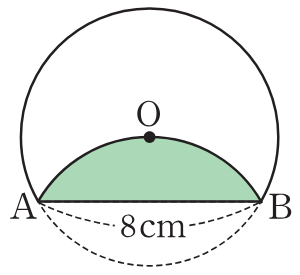
\includegraphics[width=71.9pt]{figures/fig-129-19.png}\end{minipage}\par
\begin{choicesii}{\rule[-3ex]{0pt}{8ex}$\dfrac{64}{9}\pi\mkern3mu \mathrm{cm}^2$}{\rule[-3ex]{0pt}{8ex}$\left(\dfrac{32}{9}\pi+8\sqrt{3}\right)\mathrm{cm}^2$}{\rule[-3ex]{0pt}{8ex}$(8\pi-4\sqrt{3})\mkern3mu \mathrm{cm}^2$}{\rule[-3ex]{0pt}{8ex}$\left(\dfrac{64}{9}\pi-\dfrac{16\sqrt{3}}{3}\right)\mathrm{cm}^2$}{\rule[-3ex]{0pt}{8ex}$(32\pi-4\sqrt{3})\mkern3mu \mathrm{cm}^2$}\end{choicesii}
